\documentclass[a4paper, 11pt, spanish]{article}
\usepackage[spanish, mexico]{babel}
\usepackage[utf8]{inputenc}
\usepackage{graphicx}
\usepackage{epstopdf}
\usepackage{csquotes}
\usepackage{booktabs}
\usepackage{helvet}
\usepackage{mathptmx}
\usepackage[margin=1.25in]{geometry}
\usepackage{upquote}
\usepackage{spreadtab}
\usepackage{import}
\usepackage{sectsty}
%%%%%%%%%%%%%%%%%%%%%%%%%%%%%%%%%%%%%%%%%%%%%%%%%%%%%%%%
\usepackage[dvipsnames]{xcolor}
\definecolor{azulOscuro}{rgb}{0.0, 0.28, 0.67}
\definecolor{verdeCopado}{rgb}{0.13, 0.55, 0.13}
%%%%%%%%%%%%%%%%%%%%%%%%%%%%%%%%%%%%%%%%%%%%%%%%%%%%%%%%
\usepackage[acronym, toc, style=list]{glossaries}
%\usepackage[xindy, acronym, toc, style=list]{glossaries}
\makeglossaries
\loadglsentries[main]{glosario.tex}
%%%%%%%%%%%%%%%%%%%%%%%%%%%%%%%%%%%%%%%%%%%%%%%%%%%%%%%%
\usepackage{appendix}
\allsectionsfont{\normalfont\sffamily\bfseries}
\renewcommand{\appendixname}{Anexo}
\renewcommand{\appendixtocname}{Anexo}
\renewcommand{\appendixpagename}{\normalfont\bfseries Anexo}
\usepackage{etoolbox} % we load it for the workaround
% workaround
\makeatletter
\appto{\appendices}{\def\Hy@chapapp{Appendix}}
\makeatother
%%%%%%%%%%%%%%%%%%%%%%%%%%%%%%%%%%%%%%%%%%%%%%%%%%%%%%%
\usepackage{listings}
\input{headerlisting.tex}
%%%%%%%%%%%%%%%%%%%%%%%%%%%%%%%%%%%%%%%%%%%%%%%%%%%%%%%
\usepackage{tikz}
\usepackage{setspace}
\usepackage{hyperref} % Es para la url o el indice
\hypersetup{
	colorlinks=true,
	linkcolor=black,
	citecolor=verdeCopado,
	filecolor=PineGreen,
	urlcolor=azulOscuro,
	linktoc=all,
	pdftitle={Informe de proyecto 1}
}
\usepackage{cite}
\usepackage{apacite}
\bibliographystyle{apacite}
\AtBeginDocument{
	\renewcommand{\BBOP}{[}
	\renewcommand{\BBCP}{]}
}

\input{init_caratula.tex}
\usepackage{wrapfig}

\newcommand{\code}[1]{\mbox{#1}}

\begin{document}
	\renewcommand\refname{Referencias}
	\hypersetup{pageanchor=false}
	\maketitle
	\tableofcontents % indice de contenidos
	\addtocontents{toc}{\protect\thispagestyle{empty}}
	\clearpage
	\hypersetup{pageanchor=true}

	\setcounter{page}{1}
	\section{Introducción}
% TODO: insertar chamu sobre sistemas similares disponibles, etc.
En el ámbito universitario resulta necesario mantener informadas a las personas sobre una amplia variedad de hechos, noticias y acontecimientos que sucedieron o sucederán, desde la ubicación de un aula hasta la notificación de la cancelación de una clase. Muchas veces estas notificaciones son sobre cuestiones muy efímeras, lo que requiere rapidez para empezar a transmitirlas y facilidad para tener el alcance necesario.

En las facultades de la Universidad Nacional de La Plata se consumen muchos recursos para cumplir este fin, a través de afiches, pancartas, panfletos, etc. los cuales, pese a ser de barata fabricación, no tienen una vida útil muy extensa. Además todas estas formas de comunicacion se basan en el uso de papel, que tras ser utilizado debe desecharse debido a la imposibilidad de reutilizarlo, generando una cantidad de residuos significativa. Si se tiene en cuenta que también generan una polución visual considerable, por la gran cantidad de estos distribuidos en todos los lugares transitables, resulta prudente considerar una nueva forma de comunicación.

% TODO: Mencionar sobre otros carteles comercialmente disponibles
Surge así la idea de desarrollar de un cartel electrónico reutilizable, capaz de ser configurado remotamente por las autoridades competentes, con el fin de proveer una forma de comunicación masiva más limpia, clara y menos dañina para el medio ambiente.

En este informe se describe todas las fases del desarrollo de un proyecto para la asignatura Taller de Proyecto 1. El proyecto consiste en el diseño y desarrollo de un sistema de cartel luminoso cuyo contenido es configurable de forma remota. El cartel tiene conectividad WiFi, con lo que es capaz de formar parte de una red IP.

El proyecto utilizó un proceso de desarrollo de cascada, como se muestra en la figura \ref{fig:waterfall}.

\begin{figure}[!htbp]
	\centering
	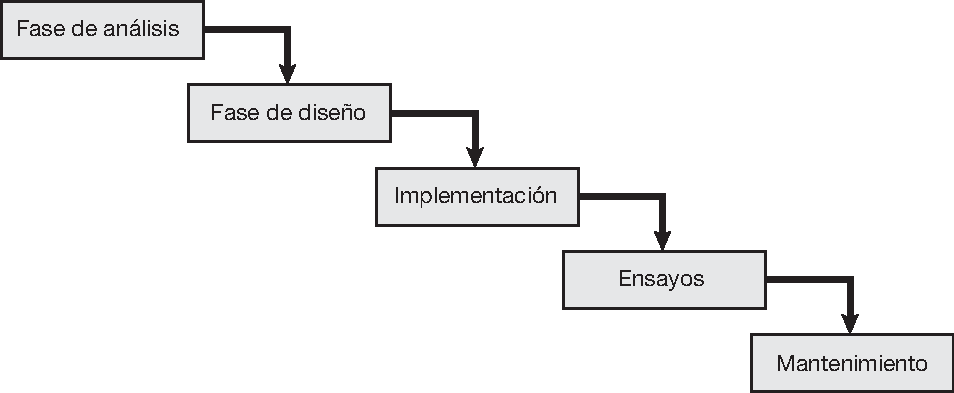
\includegraphics[width=0.8\linewidth]{imagenes/waterfall.pdf}
	\caption{Modelo en cascada de desarrollo.}
	\label{fig:waterfall}
\end{figure}

A lo largo de este informe se documentarán las fases de desarrollo previamente mencionadas.

En la sección \ref{part:analisis} se habla sobre los requerimientos y especificaciones del sistema, detallando que funcionalidades debe tener y a cuáles restricciones está sujeto.

Luego, en la sección \ref{part:diseno}, se mencionan las componentes que constituyen el sistema, se explicitan modelos que describen el comportamiento del sistema, la interfaz de usuario y la arquitectura del software. También se muestran los esquemáticos que especifican la conexión de los componentes.

En la sección de implementación se documenta como se fue dando el proceso de desarrollo de software y la implementación física del hardware.

En la sección de ensayos se documenta los resultados de las pruebas que se realizaron sobre el sistema en funcionamiento.

Por último, se anexa como apéndice una guía instructiva que explica los pasos necesarios para poner en marcha el sistema.

\section{Objetivos del proyecto}
El objetivo primario de este proyecto es el diseño implementación de un cartel luminoso que pueda ser configurado remotamente por un usuario. No se tiene como objetivo realizar un producto diseñado de manera que sea económicamente viable producirlo en masa, sino más bien el desarrollo de un prototipo a modo de prueba de concepto.

El objetivo puede ser divido en los siguientes subobjetivos:
\begin{itemize}
	\item Diseño general de la solución.
	\item Diseño e implementación del hardware que controla el cartel.
	\item Diseño e implementación del software mediante el cual se establece el contenido del cartel de forma remota.
	\item Diseño e implementación del protocolo de comunicación por el cual interactuarán las componentes.
\end{itemize}

En la parte \ref{part:analisis} se explicitará las funcionalidades que debe tener el sistema y la interfaz de usuario que expone.

\clearpage
\part{Análisis de requerimientos}\label{part:analisis}
\section{Requerimientos}
\subsection{Funcionales}
\begin{itemize}
	\item La aplicación de escritorio deberá ser capaz de poder iniciar una conexión segura con el sistema utilizando la misma para enviar los mensajes que el cliente desee.
	\item La aplicación podrá enviar peticiones de forma de obtener el mensaje actual del cartel o incluso establecer uno nuevo. Por otra parte, también podrá pedir los datos de la red a la que el sistema estará conectado o cambiarlos.
	\item La aplicación deberá ser capaz de modificar parámetros de animación tales como frecuencia de parpadeo y velocidad de desplazamiento lateral o estaticidad.
	\item La aplicación permitirá al usuario, ingresar por teclado el mensaje que desea mostrar mediante los caracteres que se establecen en el estándar de codificación de caracteres ISO/IEC 8859-1 (ver \cite{CodifChar}).
	\item El cartel deberá poder procesar sólo mensajes a través del protocolo diseñado específicamente para este proyecto (ver sección \ref{sec:protocolo})
	\item El cartel deberá mostrar los mensajes que desee el usuario.
	\item El cartel deberá poder almacenar y modificar sus credenciales de red de forma de poder conectarse al WiFi que el cliente desee.
	\item El cartel deberá mantener los datos de configuración y del mensaje que muestra, aún cuando el mismo haya sido desconectado de la red inalámbrica o de la red eléctrica.
\end{itemize}

\subsection{No funcionales}
\begin{itemize}
	\item El tiempo de respuesta del cartel no debe exceder los cinco segundos.
	\item El sistema entero no debe consumir mas de 30 Watts bajo operación normal.
	\item El sistema deberá ser capaz de aceptar sólo conexiones por TLS \cite{TLS} de forma que las conexiones y el intercambio de paquetes sea cifrado y seguro.
\end{itemize}
% TODO: Hacer diagramas de caso de uso
\subsection{Interacción con el usuario}
\section{Especificaciones físicas}
\clearpage

\part{Diseño}\label{part:diseno}
\section{Software}
\subsection{Interacción PC-Cartel}
\begin{figure}
	\centering
	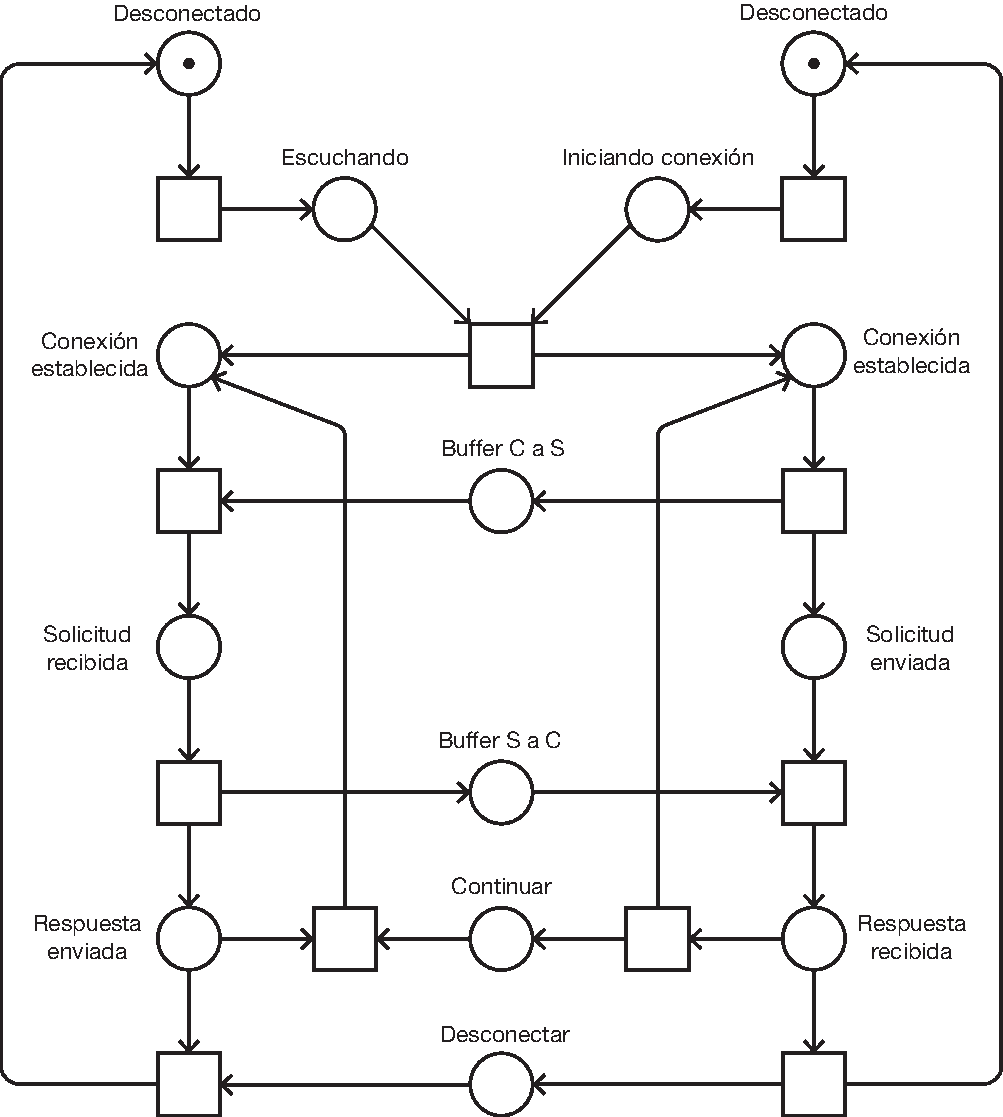
\includegraphics[width=\linewidth]{imagenes/petri-net.pdf}
	\caption{Red de Petri modelando la interacción entre la aplicación de escritorio y el cartel.}
	\label{fig:petri-net}
\end{figure}
\subsection{Firmware}
\subsubsection{Arquitectura de software}
\subsection{Aplicación de escritorio}
\subsubsection{Arquitectura de software}
\subsection{Protocolo de comunicación}\label{sec:protocolo}
\subsubsection{Transport Layer Security}

\section{Hardware}
\subsection{Diagrama en bloques general}
\subsection{Fuente de alimentación}
\subsection{Módulo maestro}
\subsection{Módulo esclavo}
\subsection{Matriz de LEDs}
\subsection{Comunicación entre los módulos}

\clearpage
\part{Ensayos y mediciones}\label{part:ensayos}
\section{Conclusiones}
% Explicar el grado de cumplimiento de objetivos planteados para el trabajo.
% Evaluar y destacar el cumplimiento y disvíos del cronograma de tareas presentados en el informe inicial
% Describir claramente la actividad de cada integrante del grupo, evaluar las horas invertidas por cada uno y calcular las horas de ingeniería total
% Analizar el presupuesto que se ha invertido y el presupuesto final del proyecto incluyendo las horas de ingeniería consumidas.

	\clearpage
	\printglossary[type=\acronymtype, title=Siglas y acrónimos, toctitle=Siglas y acrónimos]
 	\printglossary[title=Glosario, toctitle=Glosario]

	\phantomsection
	\bibliography{biblio}

	\appendix
\clearpage
\addappheadtotoc
\appendixpage

\section{Sobre Transport Security Layer}
\lstset {
	numbers=none,
	frame=none
}
\setcounter{figure}{0}
\section{Guía de puesta en marcha}
En esta anexo se explicará paso a paso como poner en marcha el sistema. Se asume que el lector de esta guía tiene conocimientos básicos de manejo de bash en GNU/Linux.

Para proceder se necesitan los siguientes elementos:
\begin{itemize}
	\item PC corriendo Debian 9 \enquote{Stretch} con ambiente de escritorio GNOME. No es necesario que sea precisamente esta distribución de GNU/Linux pero esta guía explicara los pasos para esta distribución en particular.
	\item Un módulo maestro.
	\item Al menos un modulo esclavo.
	\item Cable Micro-USB.
	% Herramientas?
\end{itemize}

\subsection{Compilación del firmware}\label{sec:comp-firmware}
En esta sección se explicará como instalar el kit de desarrollo de software de Espressif y cómo cargar el firmware al SoC (System on Chip). Para esto es necesario instalar software para traer el repositorio git y compilar el compilador que se utilizará. El compilador es el gcc de GNU pero modificado para generar código para el procesador Tonsillica Xtensa LX106, que es el que utiliza el ESP8266EX.

\subsubsection{Compilación del toolchain}
Los comandos que comiencen con \enquote{\#} deben hacerse siendo el superusuario. Una manera de abrir una sesión es usar el comando \code{su}, que permite iniciar una sesión de bash como root, el superusuario del sistema.

Primero hay que descargar \code{git} para poder clonar repositorio (este paso también aplica para la aplicación de pc):
\begin{lstlisting}
# apt install git -y
\end{lstlisting}
Debería aparecer texto similar al siguiente:
\begin{lstlisting}
root@tpi:/home/ramiro# apt install git -y
Leyendo lista de paquetes... Hecho
Creando árbol de dependencias       
Leyendo la información de estado... Hecho
Paquetes sugeridos:
  git-daemon-run | git-daemon-sysvinit git-doc git-el git-email git-gui gitk
  gitweb git-arch git-cvs git-mediawiki git-svn
Se instalarán los siguientes paquetes NUEVOS:
  git
0 actualizados, 1 nuevos se instalarán, 0 para eliminar y 0 no actualizados.
Se necesita descargar 4.160 kB de archivos.
Se utilizarán 29,5 MB de espacio de disco adicional después de esta operación.
Des:1 http://ftp.ccc.uba.ar/pub/linux/debian/debian stretch/main amd64 git amd64 1:2.11.0-3+deb9u2 [4.160 kB]
Descargados 4.160 kB en 1s (2.162 kB/s)
Seleccionando el paquete git previamente no seleccionado.
(Leyendo la base de datos ... 148278 ficheros o directorios instalados actualmente.)
Preparando para desempaquetar .../git_1%3a2.11.0-3+deb9u2_amd64.deb ...
Desempaquetando git (1:2.11.0-3+deb9u2) ...
Configurando git (1:2.11.0-3+deb9u2) ...
\end{lstlisting}

Luego, hay que descargar el SDK NON-OS para poder generar el firmware. Existe un repositorio github con un ambiente prearmado, ya que la alternativa propuesta por Espressif es descargar una imagen de una máquina virtual con Ubuntu y las herramientas ya configuradas.

Estando en el directorio home del usuario, ejecute los siguientes comandos en secuencia:
\begin{lstlisting}
$ cd
$ git clone --recursive https://github.com/pfalcon/esp-open-sdk
$ cd esp-open-sdk
\end{lstlisting}

El paso de \code{git clone} debería producir la siguiente salida:
\begin{lstlisting}
ramiro@tpi:~$ git clone --recursive https://github.com/pfalcon/esp-open-sdk
Cloning into 'esp-open-sdk'...
remote: Counting objects: 539, done.
remote: Total 539 (delta 0), reused 0 (delta 0), pack-reused 539
Receiving objects: 100% (539/539), 335.47 KiB | 296.00 KiB/s, done.
Resolving deltas: 100% (311/311), done.
Submodule 'crosstool-NG' (https://github.com/jcmvbkbc/crosstool-NG) registered for path 'crosstool-NG'
Submodule 'esp-open-lwip' (https://github.com/pfalcon/esp-open-lwip) registered for path 'esp-open-lwip'
Submodule 'esptool' (https://github.com/themadinventor/esptool) registered for path 'esptool'
Submodule 'lx106-hal' (https://github.com/tommie/lx106-hal) registered for path 'lx106-hal'
Cloning into '/home/ramiro/esp-open-sdk/crosstool-NG'...
remote: Counting objects: 33801, done.        
remote: Total 33801 (delta 0), reused 0 (delta 0), pack-reused 33800        
Receiving objects: 100% (33801/33801), 17.06 MiB | 2.39 MiB/s, done.
Resolving deltas: 100% (20003/20003), done.
Cloning into '/home/ramiro/esp-open-sdk/esp-open-lwip'...
remote: Counting objects: 236, done.        
remote: Total 236 (delta 0), reused 0 (delta 0), pack-reused 236        
Receiving objects: 100% (236/236), 495.14 KiB | 317.00 KiB/s, done.
Resolving deltas: 100% (75/75), done.
Cloning into '/home/ramiro/esp-open-sdk/esptool'...
remote: Counting objects: 1466, done.        
remote: Total 1466 (delta 0), reused 0 (delta 0), pack-reused 1466        
Receiving objects: 100% (1466/1466), 4.97 MiB | 1.29 MiB/s, done.
Resolving deltas: 100% (890/890), done.
Cloning into '/home/ramiro/esp-open-sdk/lx106-hal'...
remote: Counting objects: 122, done.        
remote: Total 122 (delta 0), reused 0 (delta 0), pack-reused 122        
Receiving objects: 100% (122/122), 179.61 KiB | 0 bytes/s, done.
Resolving deltas: 100% (51/51), done.
Submodule path 'crosstool-NG': checked out '37b07f6fbea2e5d23434f7e91614528f839db056'
Submodule path 'esp-open-lwip': checked out '8c39d2179a273553466043f388772abb6251a4ca'
Submodule path 'esptool': checked out '9dfcb350e1a91bb4641f725fc6c2f126791013ce'
Submodule path 'lx106-hal': checked out 'e4bcc63c9c016e4f8848e7e8f512438ca857531d'
\end{lstlisting}

Ahora se necesitan instalar dependencias propias del repositorio recién descargado para poder compilar las herramientas de desarrollo. Con el siguiente comando se descargarán todos los paquetes necesarios:
\begin{lstlisting}
# apt install make unrar-free autoconf automake libtool gcc g++ gperf flex bison texinfo gawk ncurses-dev libexpat-dev python-dev python python-serial sed git unzip bash help2man wget bzip2 libtool-bin -y
\end{lstlisting}

Este paso puede tardar mucho o poco dependiendo de la velocidad de la conexión a Internet.

Una vez descargados todos los componentes, ingrese el siguiente comando para iniciar la compilación de las herramientas, asegurandose de {\bfseries no} ser el superusuario:

\begin{lstlisting}
$ make standalone=n
\end{lstlisting}

El makefile de este repositorio ofrece dos alternativas al momento de compilar las herramientas: si se utiliza \code{standalone=y} entonces las cabezeras y archivos objetos privativos de Espressif se acoplan al compilador, lo cual hace que no sea necesario especificar al linkeador las librerías a las cuales hay que linkear. Sin embargo, esta alternativa hace dificil personalizar algunos aspectos del linkeo y, cómo se verá mas adelante, este proyecto necesita reemplazar unas de las librerías del SDK, con lo cual se utiliza en este caso \code{standalone=n}.

Este paso toma desde 30 minutos a 2 horas, dependiendo de las prestaciones de la computadora utilizada. Al terminar debe aparecer el siguiente mensaje:

\begin{lstlisting}
Espressif ESP8266 SDK is installed, its libraries and headers are merged with the toolchain
\end{lstlisting}


Una vez terminada la compilación, hay que realizar un paso que soluciona un problema en el que el software del cartel falla en la etapa de linkeo por no entrar en una RAM dedicada a instrucciones que utiliza el ESP8266EX. Lamentablemente no hay mucha información disponible de por qué pasa esto. Como se menciono anteriormente, el SDK es privativo y no muy bien documentado, con lo que la información que circula en Internet es un mejor caso especulativa. Este paso consiste en mover un archivo (específicamente, la implementación de la libreria estándar de C) del directorio del SDK al directorio del compilador.

Estando en el directorio \code{esp-open-sdk}, ingrese el siguiente comando:
\begin{lstlisting}
$ cp sdk/lib/libgcc.a xtensa-lx106-elf/lib/gcc/xtensa-lx106-elf/4.8.5/
\end{lstlisting}

Ahora hay que dejar el compilador y las librerías en un lugar fijo, para poder invocar a los comandos y que el código linkee correctamente.

Estando en el directorio \code{esp-open-sdk}, ingrese los siguientes comandos como root:
\begin{lstlisting}
# mkdir /opt/espressif
# mv ESP8266_NONOS_SDK_V2.0.0_16_08_10 /opt/espressif/sdk
# mv xtensa-lx106-elf/ /opt/
# touch /opt/espressif/sdk/include/user_config.h
# echo "PATH=/usr/local/sbin:/usr/local/bin:/usr/sbin:/usr/bin:/sbin:/bin:/opt/xtensa-lx106-elf/bin" >> /etc/profile
# echo "export PATH" >> /etc/profile
\end{lstlisting}

Los últimos dos pasos se encargan de que los paths de los directorios donde se encuentran las herramientas ejecutables (compilador, linkeador, etc) estén en la variable de entorno PATH. Esto es necesario para poder invocar al compiladr estando en cualquier directorio sin tener que referenciarlo con su path entero.

Reinicie la PC o máquina virtual para que los últimos cambios tomen efecto.

\subsubsection{Cambio de librería de TLS}
El módulo que implementa las conexiones TLS en el ESP8266EX tiene unos problemas de implementación que provocan que el microcontrolador se congele por completo. Este problema es reconocido por Espressif y su solución consiste en aplicar un parche al SDK que reemplaza esa librería por una alternativa.

Para descargar el parche ingrese:
\begin{lstlisting}
$ cd
$ wget http://espressif.com/sites/default/files/sdks/esp8266_nonos_sdk_mbedtls_20160718.zip
$ unzip esp8266_nonos_sdk_mbedtls_20160718.zip
\end{lstlisting}

Luego, como root:

\begin{lstlisting}
# cp -rf ESP8266_NONOS_SDK_MBEDTLS/lib /opt/espressif/sdk/
\end{lstlisting}


\subsection{Generación de certificados TLS}\label{sec:cert-gen}
Como se explicó en la sección \ref{sec:tls}, la dirección de IP que toma el dispositivo está asociada al certificado público que exhibe y por lo tanto debe ser estática. En esta sección se explicarán los pasos para, una vez decidida una dirección IP para el cartel, generar el certificado con la clave pública, además de la clave privada.

El SDK provee un script que genera automáticamente el certificado y la clave privada. La clave privada y el certificado se almacenarán en el firmware del cartel y el certificado se almacenará en el ejecutable de la aplicación de PC. Esto es porque, normalmente, los certificados están firmados electrónicamente por una \enquote{Certificate Authority} o CA. En este caso el certificado de este proyecto se denomina \emph{self-signed}, con lo que es necesario \enquote{notificar} a la aplicación de PC que ese certificado es confiable.

En el directorio \code{/opt/espressif/sdk/tools} hay un archivo \code{makefile.sh}. Este es el script que generará el certificado y clave primaria. Hay que modificar el contenido de \code{makefile.sh} para definir la IP que utilizará el cartel.

Ingrese el siguiente comando para realizar una copia de seguridad del script:
\begin{lstlisting}
$ cp makefile.sh makefile.sh.bak
\end{lstlisting}

Y luego, edite \code{makefile.sh} tomando como guía la figura \ref{fig:guia-cert}.

\begin{figure}[!hbpt]
	\centering
	\includegraphics[height=10cm]{imagenes/cert-screenshot.jpg}
	\caption{El archivo \code{makefile.sh} con los datos que hay cambiar señalados.}
	\label{fig:guia-cert}
\end{figure}

Hecho esto, ejecute:

\begin{lstlisting}
$ chmod +x makefile.sh
$ ./makefile.sh
\end{lstlisting}

Esto produce el certificado y clave privada en distintos formatos. Para el sistema solo se necesitan \code{private\_key.h}, \code{cert.h} y \code{TLS.ca\_x509.cer}. Los primeros dos se utilizan en el firmware del cartel y el último es para la aplicación de PC, con lo que no debe eliminarse ya que se utilizará mas adelante en esta guía.

\subsubsection{Compilación del firmware}
A este punto ya se pueden escribir programas para el ESP8266EX y compilarlos. Ahora falta descargar el código del software del cartel. El mismo se encuentra en un repositorio de Github.


Ingrese los siguientes comandos para descargar el código fuente del firmware y copiar el certificado y clave privada:

\begin{lstlisting}
$ cd
$ git clone --recursive https://github.com/tpi-2017/esp
$ cd esp
$ cp /opt/espressif/sdk/tools/cert.h /opt/espressif/sdk/tools/private_key.h .
\end{lstlisting}

Para compilar ingrese:
\begin{lstlisting}
$ make
\end{lstlisting}

La salida del comando \code{make} incluir lo siguiente en las últimas líneas:
\begin{lstlisting}
xtensa-lx106-elf-g++ main.o server.o message_handler.o wifi_manager.o settings.o protocolo/Message.o led_sign.o font.o -nostdlib -Wl,--start-group -lmain -lnet80211 -lwpa -llwip -lpp -lphy -lmbedtls -lc -Wl,--end-group -lgcc -L/opt/espressif/sdk/lib -Teagle.app.v6.ld -o node
esptool.py elf2image node
esptool.py v1.2
\end{lstlisting}

\subsection{Configuración del hardware}
% Nahuel y/o santi
\subsubsection{Carga del firmware}
Una vez que se han completado los pasos en la sección \ref{sec:comp-firmware}, se puede proceder a cargar el firmware al cartel ya preparado.

La carga del firmware tiene que hacerse como usuario root, pero antes de realizar la carga es necesario correr un comando extra que vuelve a definir la variable de entorno PATH para incluir a la herramienta de carga del firmware.
Para hacer esto es necesario ir hacia el directorio donde se haya descargado el firmware y correr:
\begin{lstlisting}
# source /etc/profile
# make flash
\end{lstlisting}

La salida debe ser:
\begin{lstlisting}
root@tpi:/home/ramiro/esp# make flash
esptool.py write_flash 0 node-0x00000.bin 0x10000 node-0x10000.bin
esptool.py v1.2
Connecting...
Auto-detected Flash size: 32m
Running Cesanta flasher stub...
Flash params set to 0x0040
Writing 45056 @ 0x0... 45056 (100 %)
Wrote 45056 bytes at 0x0 in 3.9 seconds (91.6 kbit/s)...
Writing 294912 @ 0x10000... 294912 (100 %)
Wrote 294912 bytes at 0x10000 in 25.7 seconds (91.9 kbit/s)...
Leaving...
\end{lstlisting}

Si el firmware se cargó correctamente, el sistema debería ya estar funcionando, conectado a la red por defecto y esperando una conexión para ser configurado.

\subsection{Compilación de la aplicación de PC}
En esta sección se mostrarán los pasos para compilar y correr la aplicación de PC.

La aplicación de PC también se encuentra en un repositorio de Github, con lo que si ya se realizó la sección anterior, no es necesario instalar git.

Para traer el repositorio ingrese:
\begin{lstlisting}
$ cd
$ git clone --recursive https://github.com/tpi-2017/Panel
$ cd Panel
\end{lstlisting}

Antes de compilar es necesario instalar las dependencias y copiar el certificado público (ver sección \ref{sec:cert-gen}):

\begin{lstlisting}
# apt install qt5-default -y
$ cp /opt/espressif/sdk/tools/TLS.ca_x509.cer res/
\end{lstlisting}

El siguiente paso es la compilación en sí:

\begin{lstlisting}
$ qmake
$ make
\end{lstlisting}

Esto producirá un archivo llamado \code{Panel}, este es el ejecutable y se puede correr haciendo:

\begin{lstlisting}
$ ./Panel
\end{lstlisting}

Con esto concluye la puesta en marcha del software del sistema.
\section{Manual de usuario} \label{sec:manual-usuario}

\subsection{Primer uso}\label{sec:primer-uso}
Para el primer uso, es necesario tener disponible una red WiFi con los siguientes parámetros. Esto se puede conseguir utilizando un celular o una notebook, configurandola como punto de acceso, como hacer esto no se cubrirá en esta guía.

\begin{description}
	\item[Nombre de red (SSID):] TP12017G7
	\item[Contraseña de red:] abcd1234
\end{description}

El cartel tomará la IP 192.168.43.254, sin importar a qué red esté conectada.

El microcontrolador cuando se prende por primera vez, tendrá un mensaje predeterminado y se conectará a la siguiente red predefinida:

La contraseña de acceso por defecto será \enquote{1234}. Ésta deberá ser modificada rápidamente en el primer uso, para evitar que un atacante lo haga antes. Este procedimiento se explica en la sección \ref{sec:guia-password}.

Como siguiente paso, se debe cambiar la red a la que se conecta el cartel a una red WiFi fija, a la que siempre se conectará el cartel al encenderse. Este procedimiento se explica en la sección \ref{sec:guia-wifi}.

%TODO completar las siguientes personas
\subsection{Uso del cartel}\label{sec:guia-uso}
\subsubsection{Conexión al cartel}\label{sec:guia-conexion}
Para conectar al cartel, simplemente abra el programa. Al abrir, lo primero que aparecerá es un diálogo pidiendo la dirección (en nombre o IP) del cartel.  Se puede ver este diálogo en la figura \ref{fig:scr-login}.

Ingrese la dirección y la contraseña y haga click en \enquote{Aceptar}. Si la contraseña es correcta, será llevado a la ventana principal de la aplicación. En caso contrario, se volverá a pedir los datos hasta que sean correctos.

\subsubsection{Cambio de contraseña de acceso}\label{sec:guia-password}
Para realizar esta acción se necesita haber ingresado previamente la contraseña de acceso y encontrarse en la ventana principal de la aplicación.

Haga click sobre el menú \enquote{Panel} y luego en {Cambiar contraseña...}. Esto abrirá la ventana diálogo de cambio de la contraseña, que se puede ver la figura \ref{fig:scr-passwd}.

Una vez en esta ventana, ingrese la nueva contraseña. Ésta no deberá ser más larga que 40 caracteres. % Esto de los caracteres me lo sque del culo. Está dado por una constante en el fuente del protocolo. Era un numero parecido.
Luego, presione \enquote{Aceptar} para realizar el cambio u \enquote{Cancelar} para cancelar.

\subsubsection{Cambio de mensaje al cartel}\label{sec:guia-texto}
Para realizar esta acción se necesita haber ingresado anteriormente la contraseña de acceso y encontrarse en la ventana principal de la aplicación.

Estando en la ventana principal de la aplicación, simplemente se debe escribir en el campo \enquote{Texto} el texto deseado. A medida que se vaya escribiendo, se indicará en la esquina inferior derecha la cantidad de caracteres restantes que se pueden escribir.

Opcionalmente se puede activar el parpadeo. Para esto haga click sobre la casilla de verificación \enquote{Parpadeo} y defina el valor de frecuencia deseado en Hertz. El mismo procedimiento aplica para la velocidad de desplazamiento.

\subsubsection{Cambio de red WiFi}\label{sec:guia-wifi}
Para realizar esta acción se necesita haber ingresado anteriormente la contraseña de acceso y encontrarse en la ventana principal de la aplicación.

Haga click sobre el menú \enquote{Panel} y luego en \enquote{Cambiar configuración de red...}. Esto abrirá un dialogo con campos editables que corresponden al nombre de red y la contraseña de la red a la cual deberá conectarse el cartel al aplicar el cambio. Se puede ver esta ventana en la figura \ref{fig:sec:guia-wifi}.

Luego, presione \enquote{Aceptar} para realizar el cambio u \enquote{Cancelar} para cancelar.

\subsubsection{Reestablecimiento de configuración}\label{sec:guia-reset}
Para realizar esta acción se necesita acceso físico al hardware.

Puede ocurrir que la red a la cual el cartel se conectaba ya no esté disponible o el administrador del cartel se haya olvidado o perdido la contraseña. En estos casos es deseable llevar el cartel a un estado conocido.

Para reestablecer la configuración del cartel, presione el botón de RESET del cartel por aproximadamente 5 segundos. Sabrá que se reinicio cuando vea parpadear el cartel y aparezca un mensaje inicial genérico. A partir de este momento, el cartel volverá a conectarse a la red especificada en la sección \ref{sec:primer-uso}.

\section{Lista de materiales}\label{sec:materiales}

\subsection{Materiales del cartel}

\subsubsection{Componentes del módulo esclavo}
Para poder armar este módulo es necesario contar con los siguientes componentes:
\begin{itemize}
    \item 64 LEDs.
    \item Un PCB con dimesiones minimas de 7x7cm.
    \item Un MAX7219.
    \item Un capacitor polarizado 10µF.
    \item Un capacitor no polarizado 0.1µF.
    \item Una resistencia 24KOhm.
    \item Dos conector hembra 8 Pin (25.4mm): para la conexión de la matriz de LEDs.
    \item Dos conector hembra 5 Pin (25.4mm): para la interfaz entre módulos.
    \item Dos regleta de 1x12 pines hembra (1.27mm): para la conexión del MAX7219.
\end{itemize}    

\subsubsection{Componentes del módulo master}
Para poder armar este módulo es necesario contar con los siguientes componentes:
\begin{itemize}
    \item Un NodeMCU Esp8266.
    \item Un PCB con dimesiones minimas de 7x7cm.
    \item Tres transistor NPN.
    \item Seis Resistencia de 10KOmh.
    \item Cuatro Jumpers.
    \item Un Jack con bornera.
    \item Una Tecla Rocker Switch.
    \item Dos Regleta de 1x15 pines hembra: para la conexión del NodeMCU.
    \item Un conector hembra 5 Pin (25.4mm): para la interfaz entre módulos.
\end{itemize}

\subsection{Materiales para hacer el cartel}\label{sec:materiales-para-hacer-cartel}

 A continuación se mensionará los materiales que fueron utilizados en la fabricación del cartel.
 En primer lugar para poder hacer el circuito PCB se opto por la técnicas de transferencia con planchado.
 Lo cual requiere una hoja A4 papel ilustración de 90g, ácido sulfúrico, soldador, estaño, plancha, cables varios para los puentes y el archivo de impresión de la figura \ref{fig:imp-pcb}.

 Como las soldaduras no son superficiales es necesario un taladro o torno con las siguientes medidas de mechas, para perforar los agujeros de:
 \begin{itemize}
     \item 0.75mm: Resistencias, capacitores, integrados, etc.
     \item 1mm: Tiras de pines.
     \item 1.25mm: Borneras y postes.
     \item 3.25mm: Tornillos.
 \end{itemize}

 \begin{figure}[ht!]
	\centering
	\includegraphics[width=\linewidth]{imagenes/hw/imp.pdf}
	\caption{Impresión PCB del módulo master y esclavo.}
	\label{fig:imp-pcb}
\end{figure}

\end{document}